\documentclass[12pt]{article}
\usepackage{geometry}
\usepackage{titlesec}
\usepackage{enumitem}
\usepackage{hyperref}
\usepackage{graphicx}
\usepackage{todonotes}
\usepackage{float}
\usepackage{amsmath}
\usepackage{tikz}
\usepackage{booktabs}
\usepackage{hyperref}
\usepackage{url}
\usetikzlibrary{positioning, shapes.geometric, arrows.meta}

\geometry{a4paper, margin=1in}
\titleformat{\section}{\large\bfseries}{\thesection}{1em}{}
\titleformat{\subsection}{\normalsize\bfseries}{\thesubsection}{1em}{}

%-------------Ttitle Page-------------
\begin{document}

\begin{titlepage}
    \centering
    \vspace*{\fill}

    {\LARGE \textbf{Final Year Project: Preliminary Report}}\\[2em]
    {\large Development of an Explainable Deep Learning Model for}\\[0.5em]
    {\large Early Breast Cancer Detection in Singaporean Women with Dense Tissue}\\[4em]

    {\large \textbf{Justin Lim}}\\[1em]
    {\large \today}

    \vspace*{\fill}
\end{titlepage}
\newpage
\tableofcontents
\newpage

%-------------Introduction Page-------------
\newpage
\section{Introduction}
\noindent\textbf{Word count:} 714
\vspace{1em}

\subsection{Project Template}
3.2 Project Idea 2: Deep Learning Breast Cancer Detection

\subsection{Background}

Breast cancer remains the most common cancer among women in Singapore~\cite{10}, accounting for approximately 29.6\% of all female cancers diagnosed between 2018 and 2022. The lifetime risk of developing breast cancer by age 75 is 1 in 12 women~\cite{10}. Early detection plays a critical role in improving survival outcomes, with five-year age-standardised relative survival (ASRS) improving from 49.9\% in the 1970s to 83.1\% in recent years~\cite{10}.

Despite the availability of population-wide screening initiatives such as BreastScreen Singapore~\cite{6}, several persistent challenges continue to limit the effectiveness of such programs. These include under-screening in older women, lower participation among specific ethnic groups, and diagnostic difficulties associated with dense breast tissue. Notably, women over 80 have a five-year survival rate of only 38.6\%, compared to 71.9\% for those aged 50--59~\cite{10}. Additionally, survival disparities persist across ethnicities, with Malay women exhibiting the lowest five-year survival rate among major ethnic groups (46.7\%)~\cite{10}.

Traditional risk models often underperform in these high-risk populations, leading to delayed or missed diagnoses. Furthermore, the interpretation of dense mammograms remains a significant clinical challenge, even for experienced radiologists. These limitations underscore the need for enhanced, explainable diagnostic tools tailored to Singapore’s population and screening realities.

\subsection{Motivation}
Deep learning models—particularly Convolutional Neural Networks (CNNs)—have shown significant promise in enhancing medical image interpretation, including breast cancer detection. Multiple studies have demonstrated their ability to outperform traditional statistical and risk based models, particularly in challenging scenarios such as high breast density~\cite{1,7,13}. However, most of these models are developed using Western datasets, making them less effective or generalizable in a Southeast Asian context.

Moreover, clinical adoption remains limited due to the ``black-box'' nature of deep learning models. Trust is a key barrier clinicians are unlikely to rely on algorithmic outputs without transparent decision making. Explainable AI techniques like Gradient weighted Class Activation Mapping (Grad-CAM)~\cite{5} address this challenge by offering visual explanations of model decisions. These heatmaps show which regions of an image contributed most to the model's prediction, enabling radiologists and clinicians to verify AI-generated insights.

This project is therefore motivated by two key needs: (1) to improve breast cancer detection in under screened, high risk Singaporean women using localized AI models; and (2) to enhance trust and usability in clinical workflows through model explainability.

\subsection{Project Concept}
This project proposes an \textbf{explainable deep learning system} for the classification of mammography and histopathology images to assist in breast cancer diagnosis. The system is designed to address local screening gaps by focusing on high risk features such as dense breast tissue and older age profiles.

The core of the system is a CNN based model (e.g., ResNet~\cite{17} or EfficientNet), trained to classify input images into benign or malignant categories. It will be developed using publicly available datasets, preprocessed and adapted to reflect local imaging characteristics.

To promote transparency, the system incorporates \textbf{Grad-CAM}~\cite{5} as a post hoc interpretability tool. This technique will generate heatmaps over input images, highlighting areas most influential in the model’s predictions. These visual explanations are crucial for ``human-in-the-loop'' workflows, where clinicians can evaluate and validate AI assisted diagnostics. In practice, this supports both improved diagnosis and user confidence in the tool.

\subsection{Project Objectives}
\label{sec:objectives}
The key objectives of this project are:
\begin{itemize}
    \item {Model Accuracy:} To develop a CNN-based image classification model that achieves at least {85\% accuracy} in detecting breast cancer from mammography and histopathology images.
    \item {Robustness on Local Profiles:} To ensure robust performance, particularly in {dense breast tissue and older age groups}, by maintaining {sensitivity above 80\%} across those subgroups, reflective of Singaporean demographics.
    \item {Explainability:} To generate {Grad-CAM visualizations} that consistently highlight diagnostically relevant regions, enabling human verification and supporting model transparency.
\end{itemize}

\subsection{Deliverables}
This project will produce the following deliverables:
\begin{itemize}
    \item {Trained CNN Model:} A fully trained and validated deep learning classification model (e.g., ResNet or EfficientNet) capable of classifying mammography and histopathology images.
    \item {Grad-CAM Visualizations:} A set of Grad-CAM heatmaps overlaid on test images to illustrate model attention and provide interpretability.
    \item {Performance Report:} A formal evaluation report detailing key classification metrics—{Accuracy, Sensitivity, Specificity, and F1-Score} across both general test sets and specific high-risk subsets.
\end{itemize}
\newpage

%-------------Literature Review Page-------------
\newpage
\section{Literature Review}
\noindent\textbf{Word count:} 2279
\vspace{2em}

This chapter reviews the limitations of traditional breast cancer risk models, the role of deep learning in diagnostic imaging, the importance of explainability, and challenges in generalizing models across diverse populations. Each section provides justification for the design choices and objectives outlined in this project emphasizing the need for a localized, explainable deep learning system in Singapore's screening context.

\subsection{Analysis of Similar Projects and Tools}

To ensure the proposed system is both technically sound and contextually relevant, it is important to review recent advancements in AI-assisted breast cancer screening. This comparative analysis highlights key successes and limitations of existing tools and research. By examining how these systems were designed, evaluated, and applied in real-world scenarios, this can identify best practices and avoid common pitfalls. This analysis also helps justify the architectural and design decisions made in this project particularly the emphasis on explainability, local adaptation, and clinician-in-the-loop deployment.

Several notable AI systems and studies in breast cancer screening have influenced this project’s design. Each offers lessons on performance, integration, and limitations that inform how the proposed prototype addresses both technical and clinical challenges specific to Singapore.

\begin{itemize}
    \item \textbf{Google Health / DeepMind – Mammogram AI System} \\
    This system, trained on over 90{,}000 mammograms, demonstrated strong diagnostic capabilities, outperforming radiologists in controlled trials~\cite{11}. However, the system's performance decreased significantly when applied to external datasets, highlighting its limited generalization capabilities. To mitigate such risks, this project incorporates stratified testing and local data simulation techniques to better represent the breast density profiles and demographic variations seen in Singapore.

    \item \textbf{Zebra Medical Vision – Scalable Cancer Detection Tools} \\
    Zebra’s AI tools gained traction due to their regulatory approval and ease of integration into existing cloud-based radiology systems~\cite{12}. While their deployment model is highly scalable, a lack of interpretability in model decisions has raised concerns about trust and transparency. To address this, the proposed system integrates Grad-CAM visualizations directly into the diagnostic output, ensuring interpretability without sacrificing operational compatibility.

    \item \textbf{Shen et al. (2019) – CNN-Based Mammogram Classifier} \\
    Shen et al. applied CNNs to mammographic image classification with encouraging results~\cite{7}, yet their work revealed an ongoing reliance on large, high-quality, annotated datasets for training. Given the challenges of acquiring such datasets locally, this project includes data augmentation techniques and a compact network architecture to maintain performance while coping with limited annotated image availability in Singapore.

    \item \textbf{Salim et al. (2024) – AI in Population-Based Screening (Sweden)} \\
    This real-world study evaluated AI deployment across over 58{,}000 mammograms in Sweden and reported improvements in screening efficiency without a loss in accuracy~\cite{13}. Despite the AI’s success, radiologists continued to play an oversight role, ensuring clinical safety. This project adopts a similar human-in-the-loop model, using AI-generated heatmaps as supportive tools to enhance but not replace expert interpretation.
\end{itemize}

\noindent \textbf{Summary of Insights and Application to This Project:} \\
From these projects, several key insights emerge: the importance of robust validation across diverse populations, the need for transparent model outputs, and the value of seamless integration into clinical workflows. These findings shape this project’s approach by ensuring the model is both interpretable (via Grad-CAM) and tuned to local breast density distributions. Furthermore, clinician-in-the-loop design is adopted to foster trust, prevent overreliance on automation, and ensure that AI predictions enhance rather than override expert judgment. By incorporating these lessons, the proposed prototype aims to strike a balance between technical performance, clinical usability, and ethical responsibility.

% \subsection{Learning from Existing Applications}

% Two existing AI-based breast cancer prediction systems were critically reviewed to guide the design of this project:

% \paragraph{Yala et al. (2019): Deep Learning Risk Model~\cite{1}.}
% Yala and colleagues developed a deep learning model using screening mammograms to improve 5-year breast cancer risk prediction. Their system outperformed traditional risk models by leveraging raw image data and integrating patient risk factors. This project draws from their method of using image-based CNNs for individualized risk scoring and handling imbalanced data distributions—challenges also present in this project’s target dataset. However, unlike their clinical integration, this project adapts the methodology to the Singaporean demographic using public datasets and augmentation.

% \paragraph{Geras et al. (2017): Multi-View Deep CNNs~\cite{8}.}
% Geras et al. proposed a high-resolution mammography system using multiple views (cranio-caudal and mediolateral oblique) to improve lesion detection. Their approach demonstrated superior diagnostic performance through spatial context modeling. Inspired by this, the current project implements a dual-view alignment stage during preprocessing to help the CNN capture inter-view correlations and better detect abnormalities in dense tissue cases—a common issue in the Singaporean female population.

% Together, these applications provided insights on multi-view input handling, risk modeling from raw images, and architectural design—supporting both the technical robustness and clinical relevance of this project.

% \subsection{Limitations of Traditional Risk Models}

% Risk prediction models~\cite{1} form the foundation of clinical decision-making in early breast cancer detection. Conventional tools, such as the Gail and Tyrer-Cuzick models~\cite{1}, have been widely adopted in clinical settings for population-level risk stratification. These models use structured demographic and clinical inputs to estimate cancer risk but are limited by their rule-based design and assumptions of feature independence.

% For this project, understanding the limitations of these traditional models is crucial—they underscore the need for more individualized and image-informed approaches. These models are unable to capture spatial or visual features present in medical images, which are essential when diagnosing cancer in women with dense breast tissue.

% A key study~\cite{1} compared the Tyrer-Cuzick model with CNN-based deep learning models trained directly on mammograms. The deep learning models significantly outperformed the clinical models, with AUC values ranging from 0.68 to 0.70 compared to 0.62. These results were especially compelling for dense breast tissue subgroups—directly aligning with this project’s target population of Singaporean women, who often present with dense tissue at younger ages~\cite{6}.

% Appendix Figure~\ref{fig:lit1table2} ~\cite{1} further illustrates these findings. It shows that the deep learning model identified over 31.2\% of future cancers within the highest-risk decile—almost double the detection rate of the Tyrer-Cuzick model, which captured only 18.2\%. This performance gap highlights not just improved sensitivity, but also the model’s utility in stratifying high-risk cases early—an essential capability for any national screening program.

% Beyond performance metrics, traditional models are inherently limited in adaptability and interpretability. They cannot be fine-tuned for local demographics or provide spatial reasoning about predictions. For instance, local analysis~\cite{6} found that the Tyrer-Cuzick model underestimates risk in Singaporean women, leading to reduced screening recall rates and delayed diagnoses. This directly supports this project’s motivation to build a CNN-based pipeline that can be trained and evaluated using regional risk profiles.

% By shifting from predefined questionnaire-based inputs to deep, image-based learning, this project enables the model to extract and prioritize risk signals that are visually embedded in mammograms. Furthermore, with the integration of Grad-CAM, the proposed system will offer transparency in predictions—something traditional risk models fundamentally lack.

% In summary, the weaknesses of traditional models in both predictive power and adaptability strongly support the development of an explainable, localized CNN-based model tailored for dense tissue scenarios in Singapore.

\subsection{Role of Deep Learning in Breast Cancer Imaging}

To justify the deep learning approach used in this project, it is essential to examine how convolutional neural networks (CNNs) have enhanced breast cancer diagnostics. Unlike traditional models that rely on structured variables such as age and family history, CNNs operate directly on full field mammograms. This enables them to detect complex spatial features such as tissue asymmetry, mass shape, and density patterns that often precede clinical symptoms. These characteristics are particularly critical in screening contexts involving dense breast tissue, a trait common among women in Singapore~\cite{6}.

Evidence from Yala et al.~\cite{1} offers strong justification for the adoption of CNN-based image analysis as the foundation of this project. In their study, three models were compared: the Tyrer-Cuzick clinical risk model, a CNN-based image-only model, and a hybrid model combining clinical and imaging features. Both deep learning models outperformed the traditional approach, with the hybrid model achieving the highest detection rates especially among patients with dense breast tissue. Appendix Figure~\ref{fig:hybrid_density} demonstrates that these CNN-driven models captured significantly more cancers in high-risk, dense-tissue populations. This highlights the advantage of CNNs in extracting detailed visual patterns and supports their role as the core architecture for this project’s predictive pipeline.

Moreover, the hybrid model in Yala et al.~\cite{1} which combines image features with clinical metadata demonstrated marginal performance improvements over the image only CNN. For this project, this suggests that integrating additional patient specific factors (e.g., breast density or age) into the pipeline could enhance model calibration for local populations. This aligns with the desired outcome of increasing detection performance specifically in Singaporean women, where dense tissue and age related diagnostic delays are prevalent~\cite{6,10}.

Shen et al.~\cite{7} further reinforce this direction by showcasing the use of CNNs in generating Grad-CAM-based heatmaps that highlight diagnostically salient regions within mammograms. These visualizations not only aid radiologists in understanding the rationale behind predictions but also reduce overreliance on black-box outputs. As illustrated in their study, Grad-CAM helped improve trust in AI assisted diagnostics by revealing consistent and clinically relevant attention areas. This motivates the project's focus on incorporating visual explainability as an interpretability layer over CNN predictions, ultimately supporting clinician adoption.

Taken together, these works justify the technical foundations of this project: selecting CNN-based models for their spatial learning capacity, exploring hybrid architectures for incremental performance gain, and embedding explainability to facilitate clinical acceptance in the Singaporean screening context~\cite{1,6,7}.

\subsection{Explainability in Medical AI}

While deep learning (DL) models have achieved strong performance in medical imaging, their “black box” nature remains a major barrier to clinical adoption. Unlike traditional models with clearly defined features, CNNs often produce predictions without transparent reasoning. In high stakes domains like cancer diagnosis, this lack of interpretability poses ethical, legal, and practical concerns especially when errors may result in misdiagnosis or delayed treatment~\cite{3}.

This issue is particularly relevant to this project, which targets breast cancer screening in Singapore. Clinicians need to understand how and why a model makes a prediction in order to trust and act on it. As highlighted by Ching et al.~\cite{3}, explainability is not just a technical add on but a prerequisite for the responsible use of AI in healthcare. Without it, medical professionals are less likely to adopt such tools, regardless of performance gains.

To overcome this limitation, this project incorporates Gradient weighted Class Activation Mapping (Grad-CAM) into its CNN architecture. Grad-CAM generates a heatmap that shows which regions of the input mammogram contributed most strongly to a model’s prediction. These visual explanations serve as interpretive cues for radiologists, helping them validate whether the model is focusing on clinically relevant structures like calcifications or asymmetries~\cite{5}.

For instance, Selvaraju et al.~\cite{5} demonstrated how Grad-CAM could be used to highlight malignancy-related areas in medical images. Appendix Figure~\ref{fig:gradcam} shows a representative output where red activation zones correspond with tumor-like regions. Such interpretability directly supports this project’s goal of clinician-aligned AI: when a model’s attention visibly aligns with known diagnostic features, trust in its predictions increases. Conversely, if the heatmap focuses on irrelevant regions, it can signal model failure or the need for retraining adding a valuable layer of quality control~\cite{5}.

This capability is especially important in the Singaporean healthcare context, where patients and providers come from diverse ethnic backgrounds, and diagnostic baselines may differ~\cite{6}. Explainable models help bridge anatomical and cultural variability by providing a shared visual rationale for risk scores. They also reduce automation bias by keeping radiologists in the loop~\cite{3}.

Moreover, integrating Grad-CAM into the system architecture allows for routine auditing and retrospective case review. This aligns with the Ministry of Health’s emphasis on accountability and traceability in AI-driven diagnostics~\cite{6}. Visual heatmaps can be logged, reviewed, and compared over time to refine both human and machine performance~\cite{5}.

In summary, explainability is not peripheral it is central to the viability of AI in breast cancer screening. By embedding Grad-CAM into the model pipeline, this project ensures that predictions are not only accurate but also interpretable, auditable, and clinically actionable~\cite{5}.

\subsection{Dataset Diversity and Generalization}

A major consideration in designing AI systems for breast cancer screening is the extent to which models trained on one population can generalize to another. Many state-of-the-art deep learning models in this domain have been trained on datasets collected from Western populations~\cite{1}. These datasets while large and well annotated reflect clinical practices, imaging modalities, and demographic profiles that differ from those in Southeast Asia.

This limitation is particularly relevant in the Singaporean context. For example, Chau et al.~\cite{6} found that Singaporean women tend to have denser breast tissue and are diagnosed at younger ages compared to their Western counterparts. Dense tissue not only increases cancer risk but also reduces the effectiveness of mammography making detection more difficult and increasing the likelihood of false negatives. Moreover, sociocultural factors such as screening hesitancy and lower awareness compound the challenge. For this project, these differences emphasize the importance of designing a model that accounts for regional characteristics.

Yala et al.’s~\cite{1} hybrid model which combines image and clinical features performs well on U.S. data, but its effectiveness in Singaporean populations is uncertain. Appendix Figure~\ref{fig:hybrid_density} shows how cancer incidence varies significantly across tissue density and risk score categories. The stratification observed in U.S. data suggests potential for image driven models to capture visual malignancy signals; however, the model must be adapted or fine tuned for local demographics to ensure meaningful predictions.

This concern is further reinforced by Raghu et al.~\cite{2}, who investigated the value of transfer learning from ImageNet in medical imaging. Their findings, shown in Appendix Figure~\ref{fig:lit2table7}, indicate that pretrained CNNs did not significantly outperform models trained from scratch. In fact, most pretrained features were overridden during fine tuning. This supports this project’s strategy to adopt a lightweight CNN architecture trained specifically on mammographic data, rather than relying on generalized features learned from non-medical domains.

Finally, the problem of dataset scarcity must also be addressed. In regions like Singapore, access to annotated medical data is limited due to privacy regulations and small population sizes. Cheplygina et al.~\cite{4} highlight the utility of alternative learning paradigms such as semi-supervised learning (SSL)~\cite{4}, multi-instance learning (MIL)~\cite{4}, and weak supervision~\cite{4}. SSL allows models to leverage large amounts of unlabeled data alongside limited labeled samples, while MIL enables training on image bags without requiring pixel-level labels. These approaches reduce dependence on manual labeling and are more viable in data-constrained settings.

This project incorporates several of these ideas: synthetic augmentation is used to simulate dense tissue variability; focal loss is employed to prioritize underrepresented malignancy cases~\cite{2}; and the architecture is designed to accommodate future integration of local data for fine-tuning. Together, these strategies ensure that the model is not only technically sound but also aligned with the demographic and infrastructural realities of Singapore.

In summary, model generalization cannot be assumed across geographic or cultural boundaries. By prioritizing localization, training flexibility, and data-efficient learning, this project builds an AI system that is clinically relevant, demographically sensitive, and adaptable to future expansions in real-world Singaporean screening programs.

\subsection{Summary of Gaps and Relevance to This Project}

The literature reveals several key limitations that shape this project’s design. Traditional clinical models lack sensitivity in dense breast tissue~\cite{1}, while many deep learning (DL) models are trained on non-local datasets~\cite{1,6}, limiting their generalizability to Singapore. Explainability remains a major barrier to clinical adoption~\cite{3,5}, and data scarcity hinders model training in small populations~\cite{4}. In response, this project adopts a CNN-based pipeline with Grad-CAM explainability, uses augmentation for dense tissue simulation, and emphasizes localization and auditability to improve both performance and clinical relevance in Singapore’s screening context.

\begin{itemize}
    \item \textbf{Gap 1: Limited Predictive Power of Clinical Risk Models}\\
    Existing tools like the Gail and Tyrer-Cuzick models rely on structured questionnaire inputs and ignore visual indicators present in mammograms. These models struggle particularly in women with dense breast tissue a common trait among Singaporean women~\cite{6}. Deep learning models~\cite{1,7} have shown stronger performance in identifying malignancy through image features. Therefore, this project adopts a CNN-based model trained on full-field mammograms to provide higher-resolution risk detection that accounts for local anatomical traits.

    \item \textbf{Gap 2: Lack of Explainability Hinders Clinical Trust}\\
    CNNs are often criticized for their opacity~\cite{3,5}. Without interpretability, clinical uptake is limited. Grad-CAM offers a partial solution by generating saliency maps aligned with diagnostic regions~\cite{5}. This project integrates Grad-CAM to ensure radiologists can visually verify AI predictions and maintain control over diagnostic decisions, addressing trust and accountability concerns in real-world deployments.

    \item \textbf{Gap 3: Western-Centric Data Limits Generalization}\\
    Models trained on Western cohorts often fail to generalize to Southeast Asian populations~\cite{6}. High-density breast tissue, screening hesitancy, and sociocultural differences alter risk profiles. This project uses stratified evaluation and region-specific augmentation strategies to simulate local data characteristics and ensure performance relevance in Singaporean women.

    \item \textbf{Gap 4: Scarcity of Annotated Data in Southeast Asia}\\
    Annotated medical imaging data is often inaccessible due to privacy laws and cohort limitations. Alternative training paradigms such as semi-supervised and weakly supervised learning have been proposed~\cite{4}. This project incorporates data augmentation and simplified CNNs with lower parameter counts to reduce the need for extensive labeled data while maintaining robustness.

    \item \textbf{Gap 5: Overreliance on Transfer Learning from Natural Images}\\
    While transfer learning is common, recent studies show that pretrained features from ImageNet are frequently overwritten during fine-tuning in medical domains~\cite{2}. This project evaluates both pretrained and scratch-trained CNN variants to determine the most effective approach under low-data, domain-specific conditions.
\end{itemize}

\vspace{0.5em}
Collectively, these gaps justify the core architecture of this project:
\begin{itemize}
    \item CNN-based image models are prioritized over questionnaire-based tools for precision screening;
    \item Grad-CAM explainability ensures clinical interpretability and user trust;
    \item Training pipelines are adapted to local demographic factors;
    \item Lightweight architectures and weak supervision accommodate Singapore's data limitations;
    \item Transfer learning is validated critically rather than assumed.
\end{itemize}

These strategies form the foundation of a culturally responsive, explainable AI pipeline optimized for breast cancer screening in Singapore.


%-------------Project Design Page-------------
\newpage
\section{Project Design}
\noindent\textbf{Word count:} 1704
\vspace{1em}

\subsection{User and Domain Context}
This project is designed for use by clinical radiologists and public health administrators within Singapore’s national breast cancer screening infrastructure. The domain focuses on AI-assisted diagnostic tools for mammogram analysis, especially among women aged 40–60 with dense breast tissue. This demographic is underrepresented in most Western training datasets, necessitating a locally contextualized system.

These users were chosen because they are directly involved in interpreting screening results and making early intervention decisions. An AI tool tailored to their needs can improve diagnostic accuracy, reduce workload, and support informed public health strategies especially in a population with unique imaging challenges like dense breast tissue.

\subsection{System Architecture}

Figure~\ref{fig:system_architecture} provides a high-level architectural overview of the proposed breast cancer risk prediction system. It highlights the key components from image preprocessing to CNN-based classification and explainability via Grad-CAM~\cite{1,5}. Presenting the system architecture upfront provides a visual anchor for the subsequent description of each module.

The pipeline begins with mammographic image input, which is first passed through a preprocessing module (elaborated in Section~\ref{subsection:Feature Engineering}) that includes standardization techniques such as grayscale conversion, normalization, and augmentation. The cleaned and normalized images are then fed into the CNN backbone (e.g., ResNet-50 or EfficientNet-B0) for feature extraction.

From here, the architecture diverges into two parallel outputs:
\begin{itemize}
    \item A prediction head that computes a cancer risk probability score (detailed in the model section).
    \item A Grad-CAM explainability module that generates visual heatmaps to highlight important diagnostic regions.
\end{itemize}

Together, these modules form a clinician-assistive diagnostic tool capable of both prediction and transparent decision support, aligning with the system’s core objectives of accuracy, interpretability, and local adaptability.

\begin{figure}[H]
    \centering
    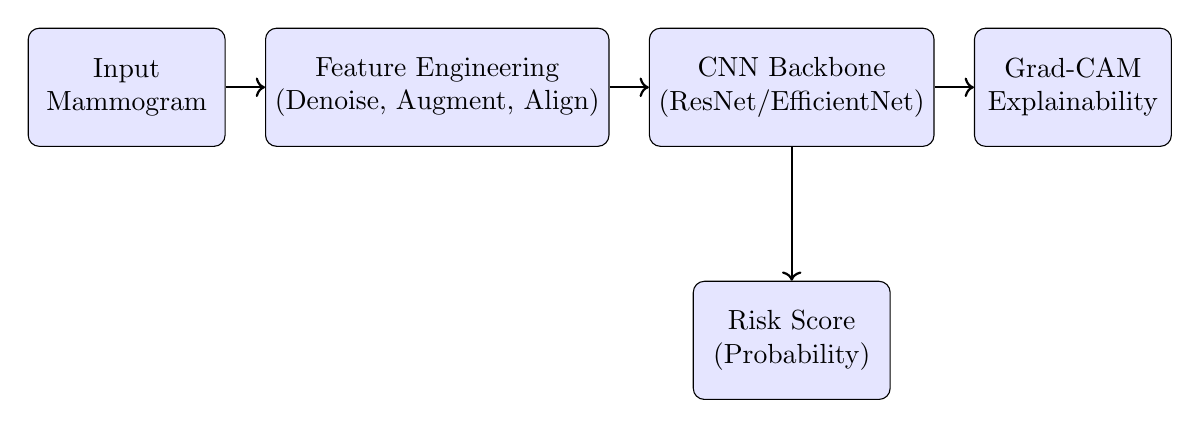
\begin{tikzpicture}[
        node distance=1cm and .5cm,
        box/.style={rectangle, draw=black, fill=blue!10, rounded corners, minimum width=2.5cm, minimum height=1.5cm, align=center},
        arrow/.style={->, thick}
        ]
        
        \node[box] (input) {Input\\Mammogram};
        \node[box, right=of input] (featureeng) {Feature Engineering\\(Denoise, Augment, Align)};
        \node[box, right=of featureeng] (cnn) {CNN Backbone\\(ResNet/EfficientNet)};
        \node[box, right=of cnn] (gradcam) {Grad-CAM\\Explainability};
        \node[box, below=1.7cm of cnn] (output) {Risk Score\\(Probability)};
        
        \draw[arrow] (input) -- (featureeng);
        \draw[arrow] (featureeng) -- (cnn);
        \draw[arrow] (cnn) -- (gradcam);
        \draw[arrow] (cnn) -- (output);
    \end{tikzpicture}
    \caption{System architecture for explainable breast cancer risk prediction using convolutional neural networks (CNNs)~\cite{1} and Grad-CAM~\cite{5}, with feature engineering integrated as a preprocessing stage.}
    \label{fig:system_architecture}
\end{figure}

\paragraph{Input Preprocessing Layer.}

Mammographic images from different sources often vary in resolution, lighting, and embedded metadata. To ensure model robustness, this stage standardizes image inputs for consistent downstream processing. Based on best practices in mammogram preprocessing~\cite{7,14}, and observations from the DDSM dataset~\cite{17}, the following steps are included:

\begin{itemize}
    \item {Grayscale conversion:} Images are converted to 8-bit grayscale to reduce computational complexity while preserving critical tissue structures.
    \item {Histogram normalization:} Applied to minimize contrast variability across acquisition devices, aiding generalization.
    \item {Resizing:} Images are resized to 224x224 pixels to match CNN input requirements~\cite{1}, enabling model reuse and compatibility.
    \item {ROI extraction:} Regions of interest are isolated by removing annotations and borders, preventing irrelevant artifacts from biasing the model. This step was adapted manually after inspecting DDSM-specific patterns~\cite{17}.
\end{itemize}

These preprocessing steps are crucial to achieving consistent input quality, especially when working with heterogeneous public datasets and simulating local screening conditions.

\paragraph{CNN Backbone.}
Feature extraction is performed using a convolutional backbone either ResNet-50 or EfficientNet-B0 chosen based on prior success in medical imaging~\cite{1,7}. ResNet-50 provides a balance of accuracy and depth, while EfficientNet’s compound scaling offers computational efficiency. Both are capable of learning fine-grained features such as mass margins, asymmetries, and microcalcifications relevant for identifying early-stage cancers in dense tissue.

This component supports the project goal of developing a model that can capture diagnostic subtleties missed by rule-based systems and generalize across patient profiles.

\paragraph{Prediction Head.}
Following feature extraction, the output is flattened and passed through fully connected layers, ending in a sigmoid neuron that outputs a cancer risk probability score. Binary cross-entropy is used as the default loss function. However, due to the class imbalance typical in screening datasets, focal loss is optionally applied~\cite{2} to improve sensitivity to rare malignancy cases—supporting early detection without overfitting on benign cases.

\paragraph{Explainability Module.}
Explainability is a design priority, not an afterthought. To address clinical transparency, Grad-CAM is integrated into the architecture. It visualizes attention maps by highlighting regions of the input image that contributed most to a model’s decision~\cite{5}. This enhances radiologists' trust and provides a layer of clinical validation—particularly important in high-density or ambiguous cases where interpretability directly impacts diagnostic decisions.

Figure~\ref{fig:system_architecture} illustrates the overall pipeline. After preprocessing, images flow through a CNN for feature extraction~\cite{1}. One branch produces a risk score; the other passes through Grad-CAM~\cite{5} to generate attention heatmaps.


\paragraph{Design Considerations.}
Each module is deliberately kept modular and swappable. This enables future expansion, such as fine-tuning on Singaporean-specific data, incorporating metadata like patient history, or using multi-view mammography inputs~\cite{8}. This architectural flexibility ensures that the system can evolve as screening datasets, clinical requirements, and deployment contexts grow more complex.

In summary, this architecture reflects a balance between predictive strength and clinical usability ensuring that both radiologists and patients benefit from a risk prediction system that is not only effective, but also transparent and adaptable.

\subsection{Dataset Used}

This project uses imaging datasets to train, evaluate, and simulate clinical performance of the proposed deep learning system. While the prototype is built using DDSM from Kaggle due to its accessibility, other datasets are reviewed to guide future enhancements for local deployment.

\paragraph{Primary Dataset – DDSM.}
The Digital Database for Screening Mammography (DDSM)~\cite{17} serves as the main dataset used for model training, testing, and prototyping. It includes over 2,600 cases with four standard views per patient (cranio-caudal (CC) and mediolateral oblique (MLO) for each breast), along with verified pathology reports and ground-truth lesion masks. Its large volume and detailed annotations make it suitable for developing convolutional neural network (CNN)-based risk prediction models. The diversity of cases—covering both normal and malignant presentations—supports effective feature learning and contrastive classification.

\paragraph{Auxiliary Dataset – BreaKHis.}
The Breast Cancer Histopathological Image Classification (BreaKHis) dataset~\cite{18} is reviewed for its potential use in future domain adaptation experiments. While it was not used in the initial prototype, it offers cellular-level detail and can be valuable for studying cross-domain robustness between mammographic and histopathological representations of breast cancer.

\paragraph{Singapore-Specific Contextualization.}
Although DDSM and BreaKHis are sourced from Western populations, this project is ultimately intended for use in Singapore. To simulate local screening challenges, future iterations of the model can incorporate demographic traits reported in the Singapore Breast Cancer Cohort~\cite{6} and the BreastScreen Singapore program~\cite{19}. These include higher prevalence of dense breast tissue and smaller breast volumes. Synthetic augmentation (e.g., increased density simulation) is used in the current model to partially approximate these traits and support contextual relevance.

\paragraph{Ethical Considerations.}
All datasets used are publicly available and de-identified, in accordance with ethical research standards. If institutional datasets from NUH or SGH are used in future development stages, formal ethics board approval will be sought prior to integration.

\subsection{Feature Engineering}
\label{subsection:Feature Engineering}

As indicated in the System Architecture (Figure~\ref{fig:system_architecture}), feature engineering is a foundational component of the preprocessing module. It ensures that raw mammographic data are transformed into a consistent and clinically enriched format suitable for CNN-based analysis. This step precedes the CNN backbone in the pipeline and directly influences both the prediction accuracy and the quality of Grad-CAM visualizations.

Figure~\ref{fig:end_to_end_pipeline} expands on this preprocessing phase in greater detail illustrating the specific transformations applied to raw DICOM images before they are passed into the CNN for feature extraction and classification.

\begin{figure}[H]
    \centering
    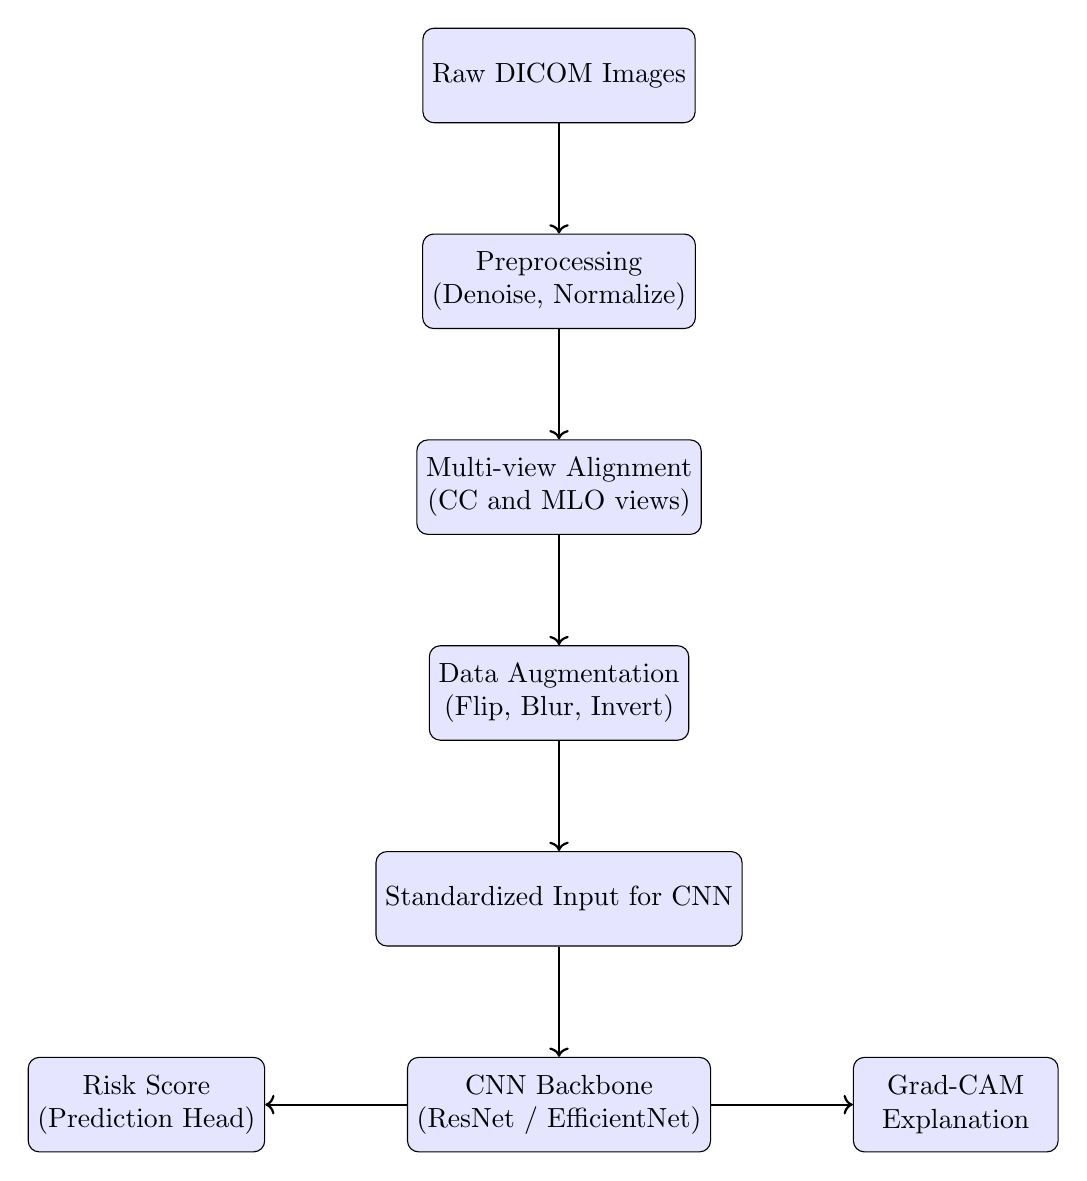
\begin{tikzpicture}[
        node distance=1.4cm and 0.8cm,
        box/.style={rectangle, draw=black, fill=blue!10, rounded corners, minimum width=2.6cm, minimum height=1.2cm, align=center},
        arrow/.style={->, thick}
        ]
        
        \node[box] (dicom) {Raw DICOM Images};
        \node[box, below=of dicom] (preprocess) {Preprocessing\\(Denoise, Normalize)};
        \node[box, below=of preprocess] (align) {Multi-view Alignment\\(CC and MLO views)};
        \node[box, below=of align] (augment) {Data Augmentation\\(Flip, Blur, Invert)};
        \node[box, below=of augment] (standard) {Standardized Input for CNN};
        \node[box, below=of standard] (cnn) {CNN Backbone\\(ResNet / EfficientNet)};
        \node[box, right=1.8cm of cnn] (gradcam) {Grad-CAM\\Explanation};
        \node[box, left=1.8cm of cnn] (score) {Risk Score\\(Prediction Head)};

        \draw[arrow] (dicom) -- (preprocess);
        \draw[arrow] (preprocess) -- (align);
        \draw[arrow] (align) -- (augment);
        \draw[arrow] (augment) -- (standard);
        \draw[arrow] (standard) -- (cnn);
        \draw[arrow] (cnn) -- (gradcam);
        \draw[arrow] (cnn) -- (score);
    \end{tikzpicture}
    \caption{End-to-end pipeline for breast cancer risk prediction, integrating preprocessing, multi-view feature alignment, CNN classification, and visual explainability.}
    \label{fig:end_to_end_pipeline}
\end{figure}

The purpose of this step is to enhance generalization and sensitivity, particularly in dense breast tissue scenarios that are common among Singaporean women. It includes denoising, contrast enhancement, multi-view alignment, and augmentation strategies—all of which standardize input images and simulate clinical variability. These processes not only improve model learning but also ensure consistency across the prediction and explainability branches of the architecture.

\paragraph{Preprocessing and Augmentation.}
The initial phase of feature engineering focuses on cleaning and enhancing the diagnostic quality of raw mammograms. This step is essential to ensure consistent model input and eliminate irrelevant imaging artifacts.

\begin{itemize}
    \item \textbf{Denoising:} Median filtering removes impulse noise (e.g., salt-and-pepper artifacts) while preserving fine structural detail important for detecting subtle anomalies like microcalcifications.
    \item \textbf{Contrast enhancement:} CLAHE (contrast-limited adaptive histogram equalization)~\cite{14} enhances local contrast, improving visibility of faint lesions, especially in dense tissue environments.
    \item \textbf{Normalization:} Pixel values are rescaled to $[0,1]$ or z-normalized to ensure uniform dynamic range, enabling more stable model convergence.
\end{itemize}

After standardization, augmentation techniques are applied to increase data diversity and improve model robustness:

\begin{itemize}
    \item \textbf{Geometric:} Random flipping, cropping, and small-angle rotations ($\pm15^{\circ}$) simulate positioning variability during imaging.
    \item \textbf{Photometric:} Gaussian blurring and contrast jitter mimic scanner inconsistencies and imaging noise.
    \item \textbf{Semantic:} Intensity inversion introduces exposure variation and histogram shifts, improving cross-device generalization.
\end{itemize}

These transformations help prevent overfitting and prepare the model for deployment across heterogeneous clinical environments.

\paragraph{Multi-View Spatial Context.}
Breast screening typically involves multiple views: cranio-caudal (CC) and mediolateral oblique (MLO). Rather than treating each view independently, this project uses a multi-view strategy to leverage spatial correlations across angles. This is based on the approach by Geras et al.~\cite{8}, who showed that multi-view CNNs improve lesion localization and diagnostic accuracy.

\begin{figure}[H]
    \centering
    \includegraphics[width=0.95\textwidth]{images/GerasFig1.png}
    \caption{High-resolution mammogram processing via multi-view deep CNNs. Adapted from Geras et al.~\cite{8}.}
    \label{fig:geras}
\end{figure}

Both CC and MLO views are preprocessed and aligned to maintain anatomical consistency. This strategy enables the model to capture bilateral asymmetries, view-dependent lesion projections, and complementary diagnostic signals critical for real-world screening reliability.

\paragraph{Domain-Specific Feature Emphasis.}
In addition to automated learning, domain knowledge is embedded to focus the model on clinically meaningful features:

\begin{itemize}
    \item \textbf{Asymmetry detection:} Breast difference maps highlight abnormal structural discrepancies between left and right sides.
    \item \textbf{Texture emphasis:} Gabor filters~\cite{20} are used to visualize texture patterns—such as spiculations—that are indicative of malignancy.
    \item \textbf{Density-informed stratification:} BI-RADS (Breast Imaging Reporting and Data System)~\cite{16} density levels are approximated via grayscale histograms and used to weight loss functions, placing more emphasis on dense cases that are diagnostically challenging.
\end{itemize}

These domain-guided strategies strengthen the model’s interpretability and diagnostic sensitivity. They also support the project’s goal of building a culturally adapted, clinically grounded AI system for breast cancer risk prediction.

\subsection{Algorithm Selection}

The choice of model architecture is guided by the need for high diagnostic accuracy, computational efficiency, and interpretability. ResNet-50 is selected as the primary benchmark due to its widespread success in medical imaging tasks~\cite{1,7}. Its use of residual connections enables deeper networks to converge efficiently while maintaining stability, making it a robust starting point for breast cancer image classification.

To explore trade-offs between accuracy, efficiency, and adaptability to medical data, two alternative architectures are also considered:

\begin{itemize}
    \item \textbf{EfficientNet-B0:} Known for its compound scaling approach, EfficientNet-B0 provides competitive performance with significantly fewer parameters than ResNet. This makes it well-suited for applications where computational resources are limited, such as deployment on hospital systems or edge devices.
    
    \item \textbf{Custom Shallow CNN:} Inspired by findings from Raghu et al.~\cite{2}, which suggest that transfer learning from large-scale natural image datasets (e.g., ImageNet) may not always benefit medical imaging tasks, a smaller model trained from scratch is included to test this hypothesis in a localized screening context.
\end{itemize}

These models were selected to support a design goal of adaptability. Depending on hardware constraints and screening requirements, different trade-offs may be acceptable. Benchmarking across these models will provide insight into the optimal balance between accuracy, efficiency, and generalization, especially for dense tissue scenarios in Singaporean women.

\paragraph{Optimization and Regularization.}
The Adam optimizer with a cyclical learning rate is used. Dropout layers are placed after the final dense layer to reduce overfitting. Early stopping with patience=10 is implemented.

\vspace{1em}

\subsection{Evaluation Metrics}

\paragraph{Quantitative Metrics.}
To evaluate model performance in a clinically meaningful way, the following metrics are selected based on their relevance to screening effectiveness, risk stratification, and imbalanced data contexts:

\begin{itemize}
    \item \textbf{AUC (Area Under the ROC Curve):} AUC reflects the model’s ability to distinguish between malignant and benign cases across all thresholds. It is used as the primary metric because it captures overall discriminability a key requirement for risk prediction tools used in screening workflows~\cite{1}. Higher AUC values indicate better model calibration across diverse patient profiles.

    \item \textbf{Sensitivity \& Specificity:} These are critical in the context of breast cancer screening, where the trade-off between detecting cancer (sensitivity) and avoiding unnecessary follow-ups (specificity) must be carefully managed. Sensitivity is prioritized in this project to reduce false negatives, particularly in dense breast tissue cases where early-stage cancers may be visually subtle and harder to detect~\cite{6}.

    \item \textbf{F1-Score:} Given the class imbalance typical in screening datasets (i.e., far fewer cancer cases), accuracy alone is insufficient. F1-score is used to provide a balanced evaluation that accounts for both precision and recall ensuring that the model not only detects cancer but does so consistently without overpredicting positives.
\end{itemize}

These metrics are selected to reflect both clinical relevance and technical robustness, aligning with the project’s dual goals of diagnostic performance and safe deployment in real-world screening contexts.

\paragraph{Explainability Evaluation.}
Grad-CAM heatmaps are overlaid on input mammograms and qualitatively scored by domain experts (when feasible) to assess alignment with tumor regions or diagnostic cues.

\begin{figure}[H]
    \centering
    \includegraphics[width=0.8\textwidth]{images/gradcam_sample.png}
    \caption{Grad-CAM visualizations showing model attention over mammograms. Red indicates regions of high diagnostic interest.}
\end{figure}

\paragraph{Qualitative Explainability Assessment.}
Beyond standard performance metrics, interpretability is essential in medical imaging. Kim et al.\ (2018) proposed the Data-driven Imaging Biomarker model (DIB-MG), which generates attention maps that highlight risk-relevant regions in mammograms. Their work supports my use of Grad-CAM as a means to validate model behavior against radiological intuition. As shown in Figure~\ref{fig:kim2018}, attention maps provide visual grounding for predictions, which is key to clinical trust and regulatory validation.

\begin{figure}[H]
    \centering
    \includegraphics[width=0.85\textwidth]{images/KimFig3.png}
    \caption{DIB-MG: Attention-based imaging biomarker model localizing high-risk regions. Adapted from Kim et al.\ (2018).}
    \label{fig:kim2018}
\end{figure}

\paragraph{Risk Stratification.}
Patients are ranked by predicted risk scores and divided into deciles. Metrics like:
\begin{itemize}
    \item \textbf{Cumulative incidence in top decile}
    \item \textbf{Hazard ratio (HR)}
    \item \textbf{Calibration curves}
\end{itemize}
are computed to evaluate clinical utility.

\paragraph{Cross-validation.}
A 5-fold stratified cross-validation is used during training. The final model is evaluated on a held-out test set to prevent data leakage and overfitting.

\vspace{1em}

\paragraph{Conclusion.}
This project adopts a structured, explainable deep learning architecture validated through standard and custom metrics. By leveraging Grad-CAM, dense tissue-aware training, and Singapore-specific context simulation, the design aligns both technically and clinically with the needs of under-screened populations in Southeast Asia.

\subsection{Work Plan and Project Timeline}

This project follows a structured timeline spanning from July to early September 2024, divided into four main phases to manage complexity, reduce risk, and ensure timely delivery. The planning was informed by a top-down decomposition of tasks based on project requirements, module interdependencies, and key submission milestones (e.g., briefing, prototype, final report). Each phase was allocated based on task duration, estimated workload, and built-in contingency.

\begin{enumerate}
    \item \textbf{Project Conceptualising (Weeks 1–5):} This phase focuses on understanding the problem domain, reviewing prior work, and preparing early deliverables (e.g., proposal video, literature review). Front-loading research activities ensures a strong theoretical foundation for later implementation.

    \item \textbf{Project Planning and Design (Weeks 5–9):} Here, the system architecture, dataset choices, and evaluation methods are formalized. Time is also allocated for early prototyping to identify technical feasibility and refine scope before development.

    \item \textbf{Development and Testing (Weeks 10–18):} The longest phase, this includes model training, iterative testing, and evaluation. Tasks are sequenced to allow progressive model improvements while maintaining checkpoints for early validation. This modular approach reduces integration risk.

    \item \textbf{Final Sprint (Weeks 18–25):} Reserved for final evaluation, report writing, and video presentation. A buffer period is also included (Week 25) to manage unexpected delays, ensuring submission readiness without compromising quality.
\end{enumerate}

Figure~\ref{fig:gantt} presents the Gantt chart visualizing these stages. The timeline not only tracks task completion but also helps balance workload over time and provides early visibility into potential bottlenecks—ensuring the project remains on schedule.

\begin{figure}[H]
    \centering
    \includegraphics[width=\textwidth]{images/PPR_GanttChart.png}
    \caption{Project Gantt chart showing planned activities from July to September 2024, divided into phases of research, design, development, and reporting.}
    \label{fig:gantt}
\end{figure}

%-------------Feature Prototype Page-------------
\newpage
\section{Feature Prototype}
\noindent\textbf{Word count:} 1792
\vspace{1em}

\subsection{Development Strategy}
This section documents the current implementation progress of the AI-powered breast cancer screening tool, referencing the modular pipeline and objectives described in Chapter 3 (Project Design).

The system was designed as a 4-stage pipeline:
\begin{enumerate}
    \item Data Preprocessing (\texttt{01\_preprocessing.ipynb})
    \item Model Training (\texttt{02\_model\_training.ipynb})
    \item Grad-CAM Visualization (\texttt{03\_gradcam\_visualization.ipynb})
    \item Evaluation (\texttt{04\_evaluation.ipynb})
\end{enumerate}

Each notebook corresponds to a critical module outlined in the system architecture. These modules are available at \href{https://github.com/justinlim00/FYP-Overview25/tree/main/FYP%20Project/FYP%20Project%20Code%20V1/notebooks}{this GitHub repository}.

The first three components were implemented in this phase because they are foundational to the system's operation and align directly with \nameref{sec:objectives} 1 and 2:
\begin{itemize}
    \item Objective 1 – Achieve high sensitivity in malignant case detection;
    \item Objective 2 – Provide visual interpretability through saliency maps.
\end{itemize}
The evaluation module is intentionally deferred to the final phase, since a working model and its outputs are prerequisites for metric-based analysis.

\subsection{Implemented Modules}
The system was developed in a staged, dependency-driven order to ensure a functional pipeline from the outset. Data preprocessing was prioritized to standardize inputs, followed by model training, interpretability, and finally, evaluation. This sequence aligns with the overall system architecture and the objectives outlined in Chapter 1.

\begin{enumerate}
    \item Data preprocessing must precede all modeling tasks.
    \item Training a working baseline model is a prerequisite for meaningful evaluation or comparison.
    \item Visualization tools (Grad-CAM) were developed early to ensure that model interpretability (Objective 2) could be validated in parallel with model accuracy.
\end{enumerate}

This prioritization ensures that the foundational system works end-to-end, allowing later additions (e.g., pretrained models, dashboard UI) to be integrated without reengineering the core pipeline.


\paragraph{\texttt{01\_preprocessing.ipynb}}
This module establishes the foundation for all downstream processing by ensuring input image consistency, format standardization, and class distribution balance. The CBIS-DDSM dataset~\cite{18} was used as the primary data source, containing curated digitized mammography images labeled with biopsy-confirmed pathology.

Key steps include:
\begin{itemize}
    \item \textbf{Grayscale Conversion:} All input PNG images were converted to grayscale to reduce channel redundancy, aligning with common practices in medical imaging literature~\cite{7}.
    \item \textbf{Size Standardization:} Images were resized to a fixed input shape of 224$\times$224 pixels to fit the input requirements of CNN architectures like ResNet and EfficientNet. This ensures model compatibility and allows efficient batch processing.
    \item \textbf{Data Structuring:} A Pandas dataframe was created to associate each image path with its corresponding label (`benign` or `malignant`), enabling seamless indexing for training and visualization workflows.
    \item \textbf{Stratified Dataset Splitting:} The dataset was split into training (70\%), validation (15\%), and test (15\%) sets using stratified sampling. This ensured that the proportion of positive (malignant) and negative (benign) samples remained consistent across all partitions, minimizing potential bias during model evaluation.
    \item \textbf{Reproducibility Measures:} Random seed values were fixed during all shuffle and split operations to ensure consistency across experiments.
\end{itemize}

The preprocessing script is modular, designed for reuse across multiple experiments. It includes parameterized options to support future image augmentation operations (e.g., rotations, contrast enhancement) in later development stages.

\vspace{0.5em}

\paragraph{\texttt{02\_model\_training.ipynb}}
This module implements the core image classification model based on a custom-designed Convolutional Neural Network (CNN). The architecture was selected for its balance between interpretability, computational efficiency, and adaptability to binary classification tasks in medical imaging~\cite{17}.

\begin{itemize}
    \item \textbf{Model Architecture:} \\
    The model begins with an input layer configured for $224 \times 224$ grayscale images with a single channel. This is followed by two sequential convolutional blocks. The first block contains a Conv2D layer with 32 filters using a $3 \times 3$ kernel and ReLU activation, followed by a MaxPooling2D layer to reduce spatial dimensions. The second block repeats this structure but with 64 filters to capture more complex patterns. After feature extraction, the feature maps are flattened into a vector and passed through a Dense layer with 128 ReLU-activated units. A Dropout layer with a rate of 0.5 is included to reduce overfitting. The final output layer consists of a single Dense neuron with sigmoid activation, designed to perform binary classification for malignant vs. benign labels.
    
    \item \textbf{Training Configuration:} \\
    The model is trained using the binary cross-entropy loss function, suitable for two-class classification problems. The optimizer used is Adam, with an initial learning rate set to 0.001, providing a good trade-off between stability and convergence speed. Training is conducted with a batch size of 32 images per step. Additionally, early stopping is applied with a patience of 5 epochs, halting training once the validation loss fails to improve, thus preventing overfitting and conserving computational resources.
    
    \item \textbf{Performance Monitoring:} \\
    Throughout training, accuracy and loss values are monitored across both training and validation datasets for each epoch. These metrics help identify signs of underfitting or overfitting as training progresses. Support for TensorBoard was also configured to visualize learning curves and performance metrics interactively, though it is optional depending on the training environment.
\end{itemize}

Initial results showed that the validation accuracy plateaued near 80\%, with slight divergence between training and validation losses in later epochs—an indication of overfitting. This behavior validates the decision to explore further enhancements such as batch normalization, learning rate scheduling, and more aggressive data augmentation in the next development cycle.

\paragraph{Handling Class Imbalance} The CBIS-DDSM dataset exhibits a skewed distribution, with benign samples outnumbering malignant ones. To address this, class weights were calculated and applied during training using Keras’s \texttt{class\_weight} parameter. This technique amplifies the contribution of minority-class (malignant) samples to the loss function, ensuring the model does not disproportionately favor the majority class. This choice directly supports Objective 1, which emphasizes early detection by maximizing sensitivity.

\paragraph{Prototype Justification} This model was chosen as the first implemented component because it establishes the diagnostic core of the system. Without a functioning classifier, neither interpretability (Grad-CAM) nor evaluation (ROC, confusion matrix) can proceed. It also lays the groundwork for future comparative experiments with pretrained networks in the final implementation.

\paragraph{Key innovation:} A threshold tuning mechanism was introduced post-training to optimize the precision–recall trade-off. This reflects clinical awareness—minimizing false negatives is more important in screening contexts than default accuracy.

\begin{table}[H]
\centering
\caption{Precision, Recall, and F1-Score at Different Thresholds}
\begin{tabular}{lccc}
\toprule
Threshold & Precision & Recall & F1-Score \\
\midrule
0.2 & 0.32 & 0.88 & 0.47 \\
0.3 & 0.40 & 0.77 & 0.53 \\
0.5 & 0.55 & 0.45 & 0.49 \\
\bottomrule
\end{tabular}
\end{table}

\paragraph{Threshold Selection Justification}
Table 1 shows that a threshold of 0.3 achieves the highest F1-score while retaining high recall. This reflects a deliberate prioritization of sensitivity, consistent with the project’s goal to reduce missed malignancies (Objective 1). Although precision drops at lower thresholds, this trade-off is clinically acceptable given the risk profile of false negatives in cancer detection.

\paragraph{Performance Implications}
At threshold 0.3, the model yielded a sensitivity of 77.05\%, precision of 40.4\%, and F1-score of 53.0\%. The ROC AUC was 0.5046. While this indicates a tendency toward overcalling malignancy, it is a valid risk-averse choice for screening. However, the modest AUC suggests poor overall discriminability, motivating the need for comparative models and further optimization in subsequent phases.

\paragraph{\texttt{03\_gradcam\_visualization.ipynb}}
This module applies Grad-CAM to visualize salient regions in classified images. Highlights:
\begin{itemize}
    \item Uses Keras backend for gradient computation and class activation map extraction;
    \item Supports overlay of color-mapped heatmaps onto grayscale mammograms;
    \item Implements enhancements such as percentile-based contrast boosting.
\end{itemize}

\textbf{Key importance:} Interpretability is central in clinical deployments. This module operationalizes Objective 2, though further improvements are needed for clinical alignment.

\begin{figure}[H]
\centering
\includegraphics[width=0.9\textwidth]{images/gradcam_grid.png}
\caption{Sample Grad-CAM overlay grid (Benign vs Malignant)}
\end{figure}

\paragraph{Interpretation:}
Figure 1 shows Grad-CAM overlays on four cases. While high-density areas are consistently highlighted, the visual attention does not always correspond to annotated tumour regions. This suggests the model may be learning general density-based features rather than fine-grained tumour morphology.

\paragraph{\texttt{04\_Evaluation.ipynb}}
Preliminary evaluation of the trained CNN model yielded the following results:

\begin{table}[H]
\centering
\caption{Evaluation Metrics on Test Set}
\begin{tabular}{lr}
\toprule
Metric & Score \\
\midrule
Accuracy & 0.4412 \\
Precision & 0.4039 \\
Sensitivity (Recall) & 0.7705 \\
Specificity & 0.2133 \\
F1-Score & 0.5300 \\
AUC & 0.5046 \\
\bottomrule
\end{tabular}
\end{table}

Table 2 reflects a strong sensitivity (77.05\%) but poor specificity, affirming the threshold trade-off decision. This prioritization of sensitivity is clinically motivated, aiming to reduce missed cancers. The AUC value of 0.5046 confirms that the model is performing only marginally better than random guessing.

\begin{figure}[H]
\centering
\includegraphics[width=0.45\textwidth]{images/confusion_matrix.png}
\caption{Confusion Matrix (Threshold = 0.3)}
\end{figure}
Figure 2 confirms this bias, with a large number of false positives contributing to the low specificity. This outcome is a direct result of the decision to shift the threshold in favor of higher recall.

\begin{figure}[H]
\centering
\includegraphics[width=0.5\textwidth]{images/roc_curve.png}
\caption{ROC Curve with AUC = 0.5046}
\end{figure}
Figure 3 visualizes the ROC curve, which shows near-random performance. This further validates the need for improved model design or fine-tuning.

\paragraph {Summary} Together, these outputs confirm the sensitivity first approach while also highlighting the limitations in model discriminability laying the groundwork for upcoming model comparisons and refinements.

\subsection{Improvements and Next Steps}
To fulfill the objectives defined in Section 1.3 and align with the architectural plan in Chapter 3, the following improvements and tasks have been identified for completion in the final phase of development:

\begin{itemize}
    \item \textbf{Model Comparison:} Thus far, only a custom CNN has been trained and evaluated. To meet Objective 3 (architecture benchmarking), additional models such as pretrained ResNet50 or VGG16 will be implemented and compared using identical data splits and evaluation metrics. This comparison will help determine whether transfer learning improves discriminability on mammography images, as expected from prior literature.

    \item \textbf{Grad-CAM Tuning and Interpretation:} Although Grad-CAM overlays have been successfully generated, they currently lack precision in localizing tumour regions. The activation maps tend to highlight broad areas rather than clearly defined features. Planned improvements include adjusting the heatmap scaling method, enhancing contrast using percentile clipping, and experimenting with different convolutional layers (e.g., earlier layers for finer texture). These changes aim to better meet Objective 2 regarding model interpretability and visual alignment with radiological expectations.

    \item \textbf{Evaluation Pipeline Finalization:} The current evaluation metrics (e.g., F1, AUC, sensitivity) have been computed manually. The final implementation will include a complete notebook (\texttt{04\_evaluation.ipynb}) that programmatically evaluates model performance at different thresholds, generates confusion matrices, and plots ROC curves. This will improve reproducibility and ensure consistency with Section 3.6.

    \item \textbf{Threshold Optimization and Reporting:} As the current model performs best at a threshold of 0.3, future work will include a grid search or Youden index strategy to determine the optimal threshold per model. Metrics at varying thresholds will be compiled into tables and compared to justify the final decision.

    \item \textbf{Objective Coverage Review:} In the final phase, each implemented feature (e.g., model accuracy, interpretability, ROC/AUC performance) will be mapped back to the specific objectives listed in Chapter 1. For example, Objective 1 emphasizes early detection through high sensitivity; Objective 2 focuses on interpretability using Grad-CAM; and Objective 3 calls for comparative evaluation of model architectures. This mapping will be summarized in the conclusion chapter.
\end{itemize}





%-------------Appendices Page-------------
\newpage
\section{Appendices}

\subsection{Figures Referenced in Section 2.1: Limitations of Traditional Risk Models}

\begin{figure}[H]
    \centering
    \includegraphics[width=\textwidth]{images/lit1table2.png}
    \caption{Performance comparison between the Tyrer-Cuzick model and deep learning models across subgroups. Adapted from [1].}
    \label{fig:lit1table2}
\end{figure}

\subsection{Figures Referenced in Section 2.2: Role of Deep Learning in Breast Cancer Imaging}

\begin{figure}[H]
    \centering
    \includegraphics[width=0.9\textwidth]{images/hybrid_risk_by_density.png}
    \caption{Cancer incidence across density groups and hybrid risk scores. Adapted from [1].}
    \label{fig:hybrid_density}
\end{figure}

\begin{figure}[H]
    \centering
    \includegraphics[height=0.7\textheight]{images/lit1_roc_auc.png}
    \caption{ROC curves comparing Tyrer-Cuzick, image-only DL, and hybrid DL models. Adapted from [1].}
    \label{fig:lit1roc}
\end{figure}

\begin{figure}[H]
    \centering
    \includegraphics[width=0.85\textwidth]{images/ShenFig2.png}
    \caption{CNN-generated detection probabilities on mammograms. Adapted from [7].}
    \label{fig:shen2019}
\end{figure}

\subsection{Figure Referenced in Section 2.3: Explainability in Medical AI}

\begin{figure}[H]
    \centering
    \includegraphics[width=\textwidth]{images/gradcam_sample.png}
    \caption{Example of Grad-CAM heatmaps overlaid on mammograms, highlighting regions associated with high-risk predictions. Adapted from [5].}
    \label{fig:gradcam}
\end{figure}

\subsection{Figures Referenced in Section 2.4: Dataset Diversity and Generalization}

\begin{figure}[H]
    \centering
    \includegraphics[width=\textwidth]{images/lit2table7.png}
    \caption{Comparison of pretrained vs. randomly initialized CNNs in medical imaging tasks. Adapted from [2].}
    \label{fig:lit2table7}
\end{figure}

%-------------References Page-------------
\newpage
\section{References}
\begin{thebibliography}{99}

    \bibitem{1}
    A. Yala, C. Lehman, T. Schuster, T. Portnoi, and R. Barzilay. 2019. A Deep Learning Mammography based Model for Improved Breast Cancer Risk Prediction. \textit{Radiology} 292, 1 (2019), 60–66. \url{https://pubs.rsna.org/doi/pdf/10.1148/radiol.2019182716}
    
    \bibitem{2}
    M. Raghu, C. Zhang, J. Kleinberg, and S. Bengio. 2019. Transfusion: Understanding Transfer Learning for Medical Imaging. In \textit{Proc. NeurIPS 2019}, 3342–3352. \url{https://proceedings.neurips.cc/paper/2019/file/eb1e78328c46506b46a4ac4a1e378b91-Paper.pdf}
    
    \bibitem{3}
    T. Ching, D. S. Himmelstein, B. K. Beaulieu-Jones, et al. 2018. Opportunities and obstacles for deep learning in biology and medicine. \textit{Nature Reviews Genetics} 19 (2018), 141–158. \url{https://royalsocietypublishing.org/doi/full/10.1098/rsif.2017.0387}
    
    \bibitem{4}
    V. Cheplygina, M. de Bruijne, and J. P. W. Pluim. 2019. Not-so-supervised: A survey of semi-supervised, multi-instance, and transfer learning in medical image analysis. \textit{Medical Image Analysis} 54 (2019), 280–296. \url{https://arxiv.org/pdf/1804.06353}
    
    \bibitem{5}
    R. R. Selvaraju, et al. 2017. Grad-CAM: Visual Explanations from Deep Networks via Gradient-based Localization. In \textit{Proc. ICCV}, 618–626. \url{https://openaccess.thecvf.com/content_ICCV_2017/papers/Selvaraju_Grad-CAM_Visual_Explanations_ICCV_2017_paper.pdf}
    
    \bibitem{6}
    W. Y. Chau, G. H. Lim, Y. L. Ng, et al. 2021. Breast density and breast cancer risk in Asian women: Evidence from the Singapore Breast Screening Programme. \textit{Cancer Epidemiology} 74 (2021), 101987. \url{https://pmc.ncbi.nlm.nih.gov/articles/PMC5160133/}
    
    \bibitem{7}
    L. Shen, L. R. Margolies, J. H. Rothstein, et al. 2019. Deep learning to improve breast cancer detection on screening mammography. \textit{Scientific Reports} 9, 1 (2019), 12495. \url{https://www.nature.com/articles/s41598-019-48995-4}
    
    \bibitem{8}
    K. J. Geras, S. Wolfson, Y. Shen, et al. 2017. High-resolution breast cancer screening with multi-view deep convolutional neural networks. \textit{arXiv preprint arXiv:1703.07047}. \url{https://arxiv.org/abs/1703.07047}
    
    \bibitem{9}
    H. J. Kim, E. Y. Ko, C. Kim, W. Han, and W. K. Moon. 2018. Applying Data-driven Imaging Biomarker in Mammography for Breast Cancer Screening: Preliminary Study. \textit{Scientific Reports} 8, 1 (2018), 12210. \url{https://www.ncbi.nlm.nih.gov/pmc/articles/PMC5807343/}
    
    \bibitem{10}
    National Registry of Diseases Office. 2022. \textit{Singapore Cancer Registry Annual Report 2022}. \url{https://www.nrdo.gov.sg/docs/librariesprovider3/default-document-library/scr-ar-2022_web-report.pdf?sfvrsn=a9eb8c10_1}

    \bibitem{11}
    S. M. McKinney, M. Sieniek, V. Godbole, J. Godwin, N. Antropova, H. Ashrafian, et al. 2020. International evaluation of an AI system for breast cancer screening. \textit{Nature}, 577 (2020), 89–94. \url{https://www.nature.com/articles/s41586-019-1799-6}

    \bibitem{12}
    Zebra Medical Vision. 2021. Zebra’s AI1 Mammography Solutions. \url{https://www.zebra-med.com/}

    \bibitem{13}
    N. Salim, J. L. Andersson, A. Nordenskjöld, H. Svensson, K. Törnberg, and K. Zackrisson. 2024. Artificial intelligence for breast cancer screening in a real-world, population-based setting: cohort study of 58,000 mammograms. \textit{Nature Medicine}, (2024). \url{https://www.nature.com/articles/s41591-024-03061-0}

    \bibitem{14}
    J. Shen, L. Margolies, J. Rothstein, E. Fluder, R. McBride, and W. Sieh. 2019. Deep Learning to Improve Breast Cancer Detection on Screening Mammography. \textit{Scientific Reports} 9 (2019), 12495. \url{https://www.nature.com/articles/s41598-019-48995-4}

    \bibitem{14}
    K. Zuiderveld. 1994. Contrast Limited Adaptive Histogram Equalization. In P. S. Heckbert (Ed.), \textit{Graphics Gems IV}, 474–485. Academic Press. \url{https://doi.org/10.1016/B978-0-08-050755-2.50065-6}

    \bibitem{16}
    American College of Radiology. 2013. Breast Imaging Reporting and Data System (BI-RADS). \textit{ACR BI-RADS Atlas, Breast Imaging Reporting and Data System}. 5th Edition. American College of Radiology.

    \bibitem{17}
    K. He, X. Zhang, S. Ren, and J. Sun. 2016. Deep Residual Learning for Image Recognition. In \textit{Proc. CVPR}, 770–778. \url{https://doi.org/10.1109/CVPR.2016.90}

    \bibitem{18}
    M. Heath, K. Bowyer, D. Kopans, R. Moore, and W. P. Kegelmeyer. 2000. The Digital Database for Screening Mammography. In \textit{Proc. 5th International Workshop on Digital Mammography}, 212–218. \url{http://www.eng.usf.edu/cvprg/Mammography/Database.html}

    \bibitem{19}
    I. A. Spanhol, L. S. Oliveira, C. Petitjean, and L. Heutte. 2016. A dataset for breast cancer histopathological image classification. \textit{IEEE Transactions on Biomedical Engineering}, 63, 7 (2016), 1455–1462. \url{https://doi.org/10.1109/TBME.2015.2496264}

    \bibitem{20}
    J. Daugman. 1985. Uncertainty relation for resolution in space, spatial frequency, and orientation optimized by two-dimensional visual cortical filters. \textit{Journal of the Optical Society of America A}, 2, 7 (1985), 1160–1169. \url{https://doi.org/10.1364/JOSAA.2.001160}
    
    \end{thebibliography}
    
\end{document}